\chapter{\fbox{TODO:CIDR Report Analysis and Observations}}
\label{chap:analysis}

The data available to conduct this analysis

\begin{figure}[H]
\begin{centering}
    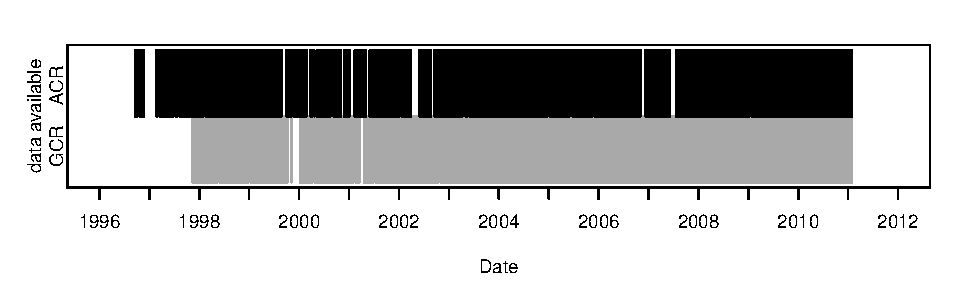
\includegraphics[width=6in]{figures/data_avail.pdf}
    \vspace{-2em}\\
    \caption{Available data}
\end{centering}
\end{figure}

\section{Characteristics of the CIDR Report}

\subsection{AS Appearances and relative measures}

Visualizations---focused on rank (a relative measure).

\begin{figure}[H]
\begin{centering}
    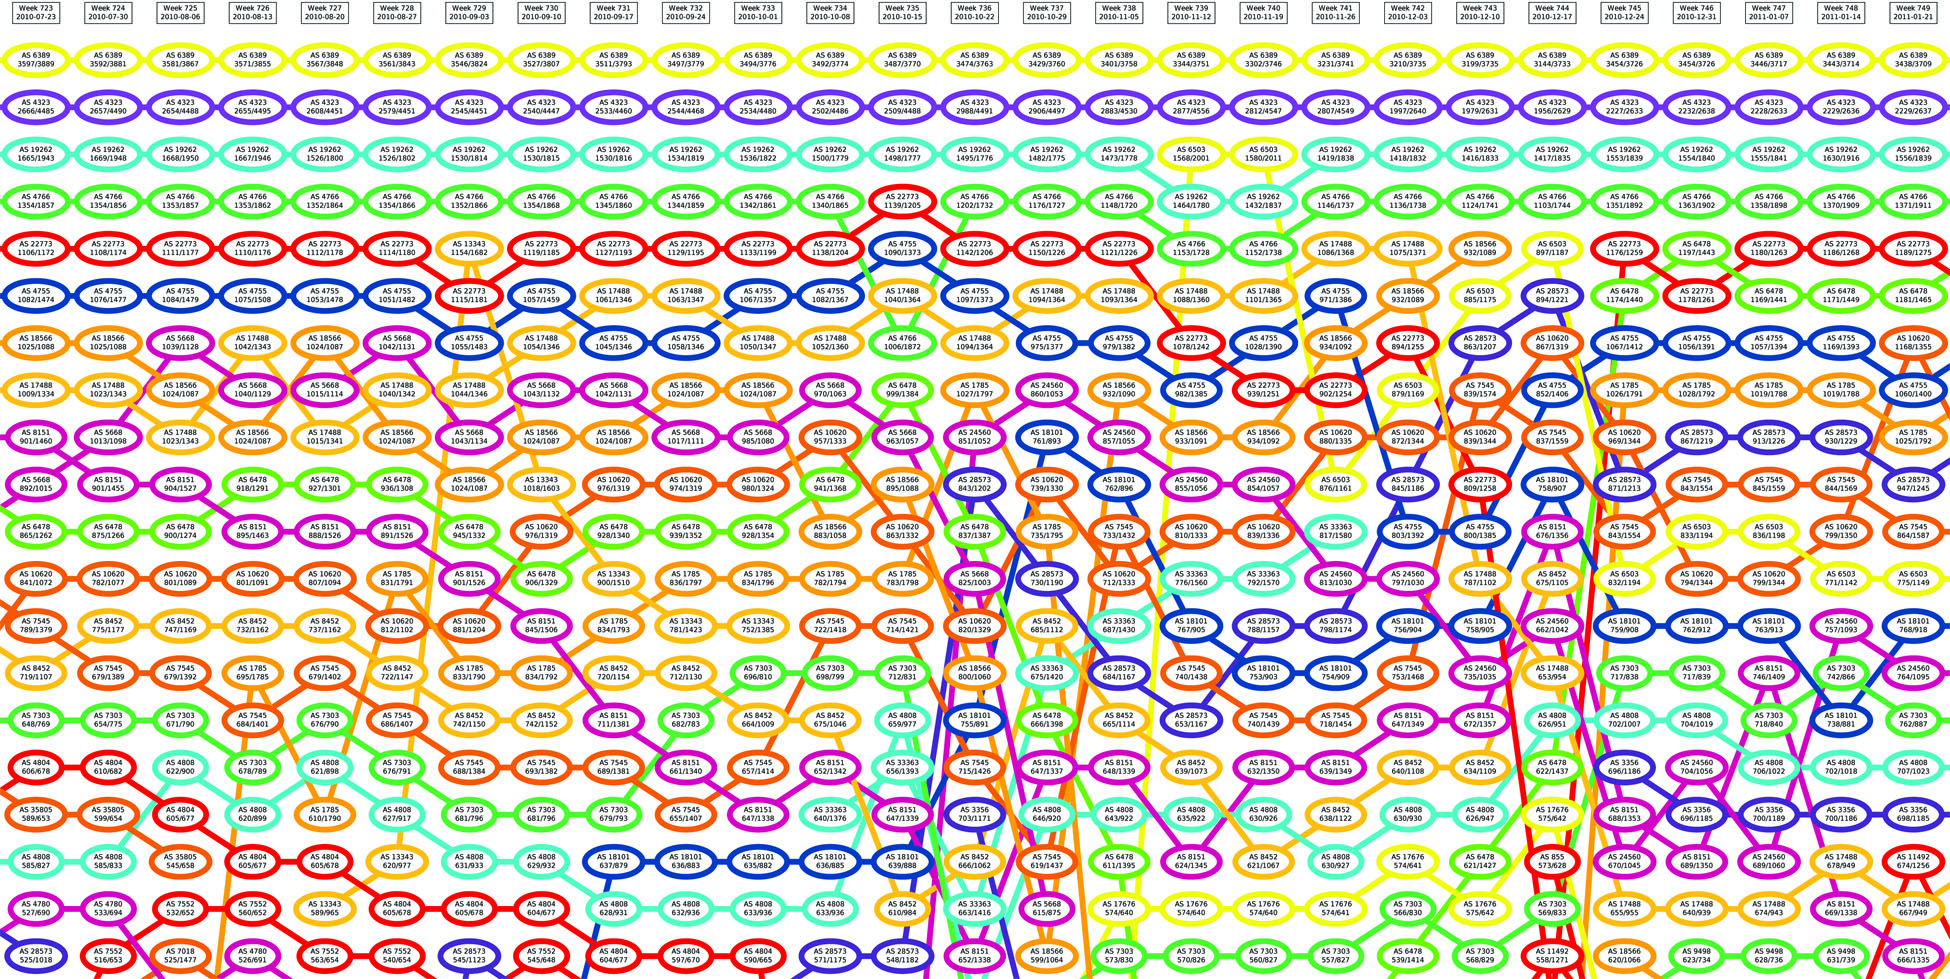
\includegraphics[width=6in]{figures/viz_sample.jpg}
    \caption{Visualization sample.}
\end{centering}
\end{figure}

These aren't very useful---let's move on to measures that are descriptive of the entire CIDR Report dataset. CDFs!

\begin{figure}[H]
\begin{centering}
    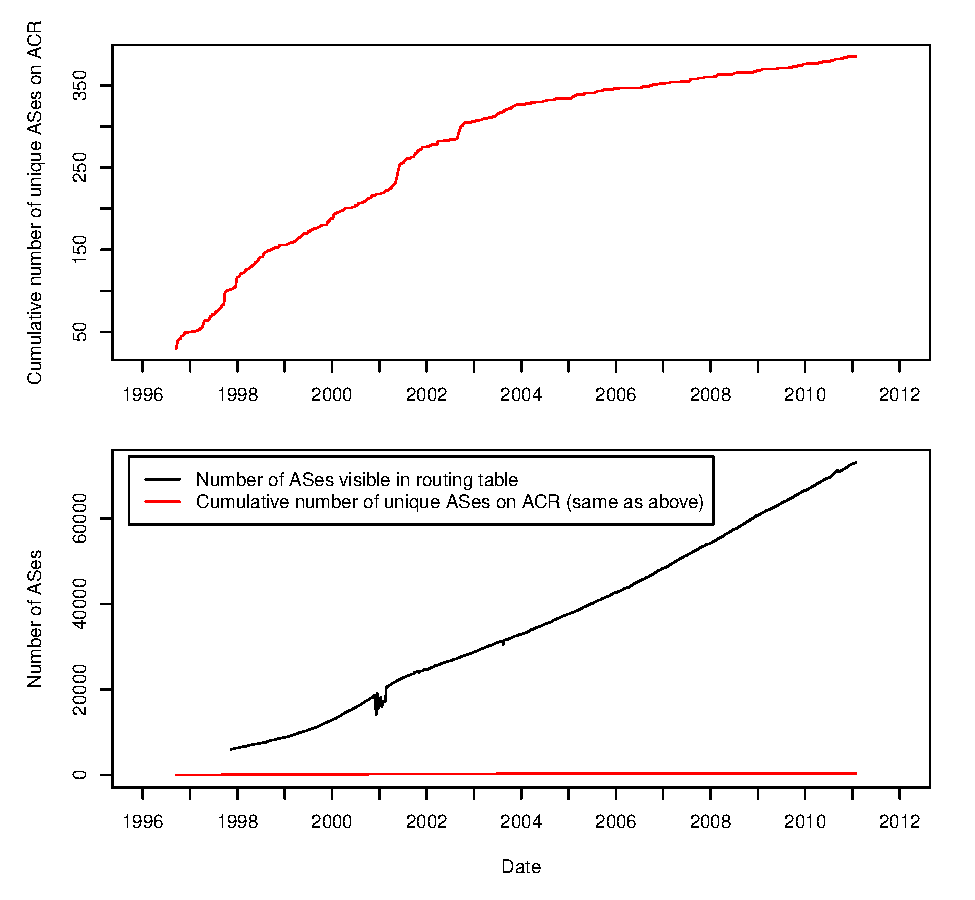
\includegraphics[width=6in]{figures/cumulative_asn_counts.pdf}
    \vspace{-2em}\\
    \caption{A cumulative count of the unique ASes that have appeared on the CIDR Report and compared to the cumulative count of unique ASes visible in the routing table up to the same point.}
\end{centering}
\end{figure}

\begin{figure}[H]
\begin{centering}
    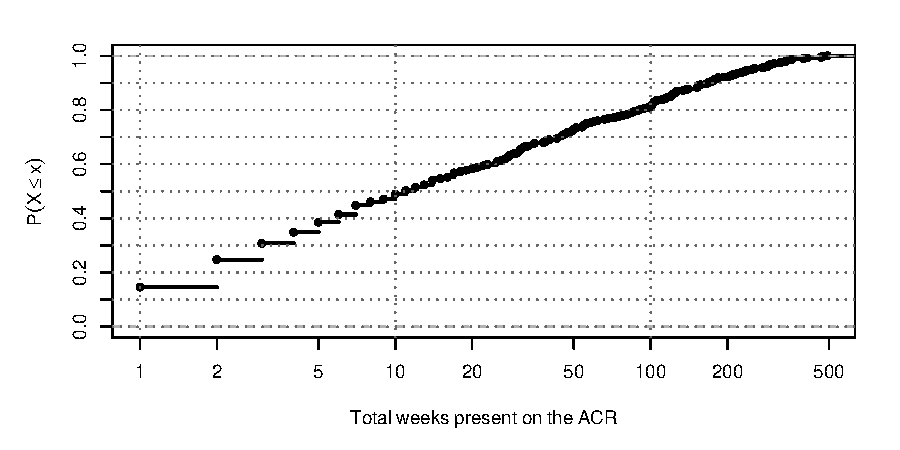
\includegraphics[width=6in]{figures/acr_cdf_weeks.pdf}
    \vspace{-2em}\\
    \caption{A cumulative distribution function of the total number of weeks that each AS is visible on the CIDR Report.}
\end{centering}
\end{figure}

\begin{figure}[H]
\begin{centering}
    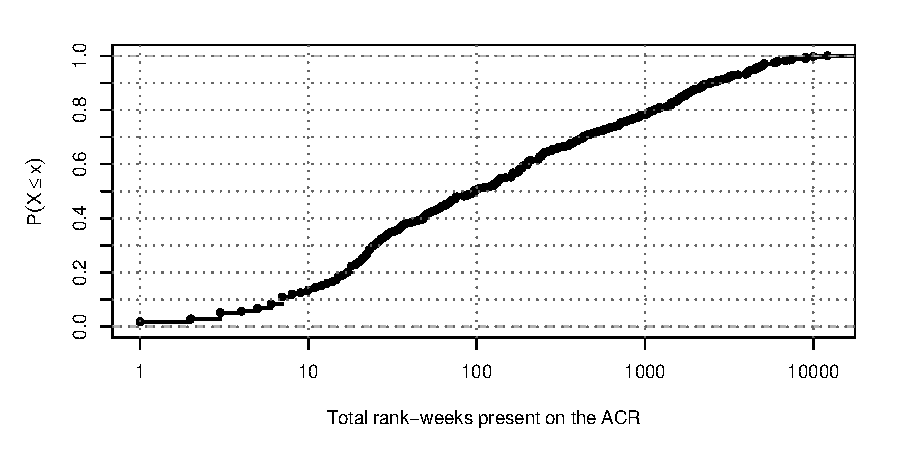
\includegraphics[width=6in]{figures/acr_cdf_rankweeks.pdf}
    \vspace{-2em}\\
    \caption{A cumulative distribution function of the total number of rank-weeks that each AS is visible on the CIDR Report.}
\end{centering}
\end{figure}

\begin{figure}[H]
\begin{centering}
    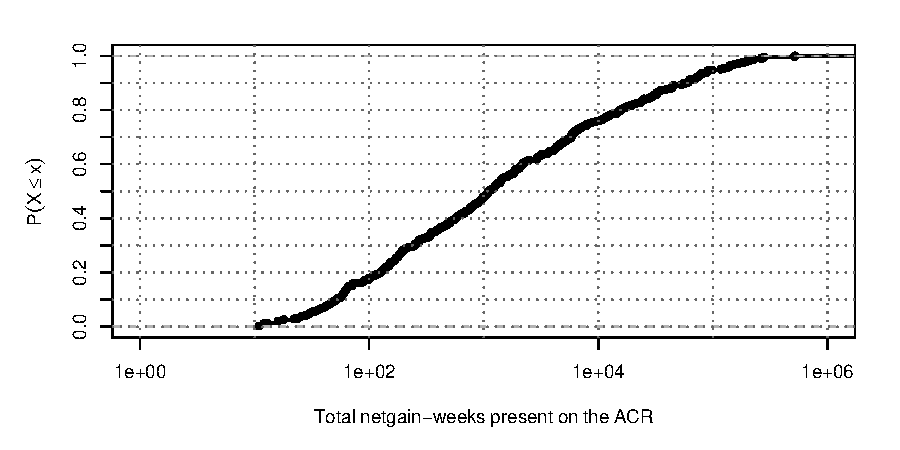
\includegraphics[width=6in]{figures/acr_cdf_ngweeks.pdf}
    \vspace{-2em}\\
    \caption{A cumulative distribution function of the total number of netgain-weeks that each AS is visible on the CIDR Report.}
\end{centering}
\end{figure}

Ok. Now let's look at CDFs of individual ASes occupying various rank slots on the ACR.

\begin{figure}[H]
\begin{centering}
    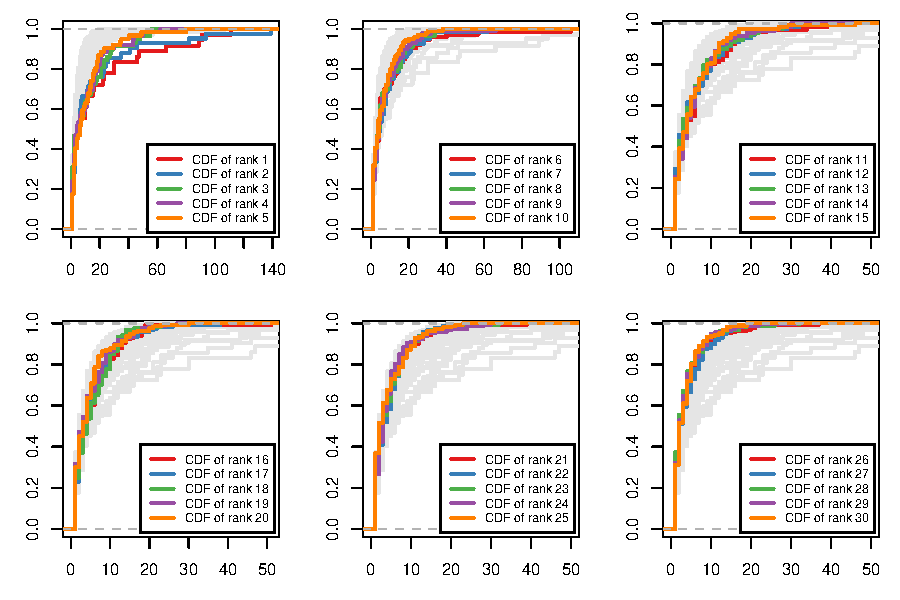
\includegraphics[width=6in]{figures/cr_rank_cdfs.pdf}
    \vspace{-2em}\\
    \caption{CDFs of the number of weeks that a given rank was occupied by a single AS. The x-axis is the number of weeks, and the y-axis is the fraction of the population. \fbox{this shows ossification/low volatility at the top}}
\end{centering}
\end{figure}

\subsection{Netgain and absolute measures}

\begin{figure}[H]
\begin{centering}
    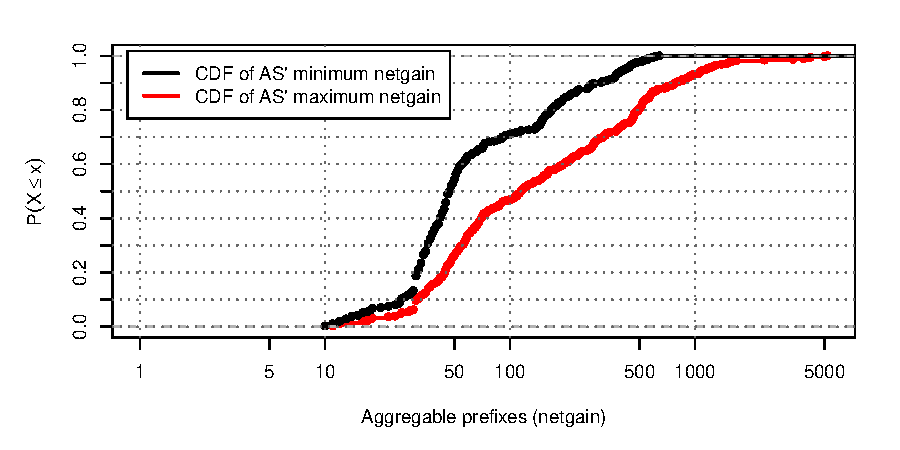
\includegraphics[width=6in]{figures/acr_netgain_cdfs.pdf}
    \vspace{-2em}\\
    \caption{CDFs of the minimum and maximum netgain observed for each AS during its time on the CIDR Report.}
\end{centering}
\end{figure}

\begin{figure}[H]
\begin{centering}
    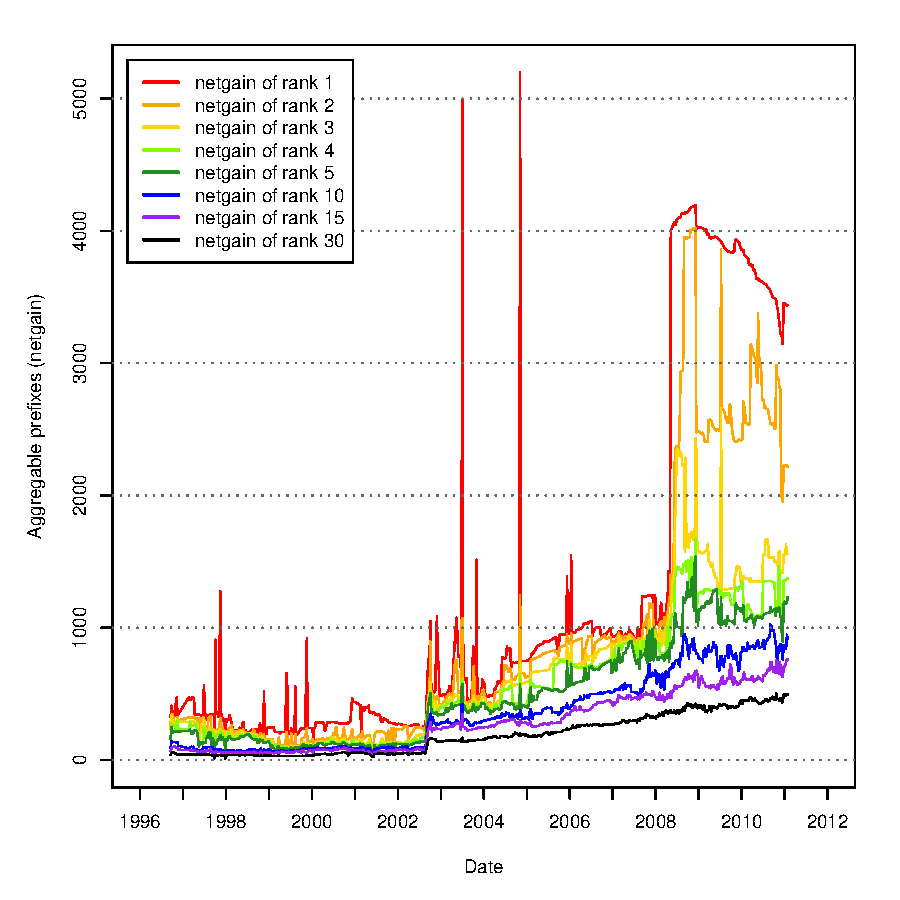
\includegraphics[width=6in]{figures/acr_netgain_time.pdf}
    \vspace{-2em}\\
    \caption{Plots of the netgain required to achieve various ranks on the CIDR Report over time.}
\end{centering}
\end{figure}

Another way of looking at the previous figure:

\begin{figure}[H]
\begin{centering}
    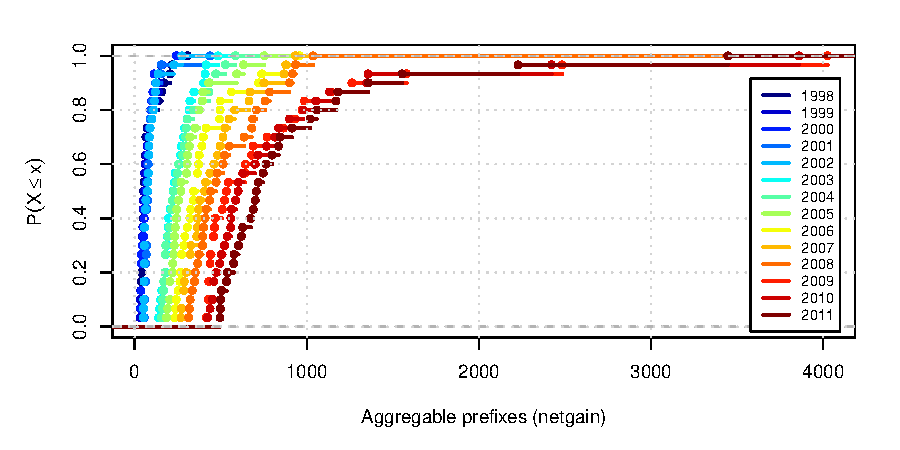
\includegraphics[width=6in]{figures/netgain_cdf_acr.pdf}
    \vspace{-2em}\\
    \caption{Plots of CDFs of the netgain of the ASes visible on the ACR in the first week of each year 1998-2011. Notice that the top of the population spreads more in later years. In other words, this is the dynamic range of the CIDR Report. \fbox{Also, don't forget about netgain\_cdf\_gcr.pdf}}
\end{centering}
\end{figure}

\begin{figure}[H]
\begin{centering}
    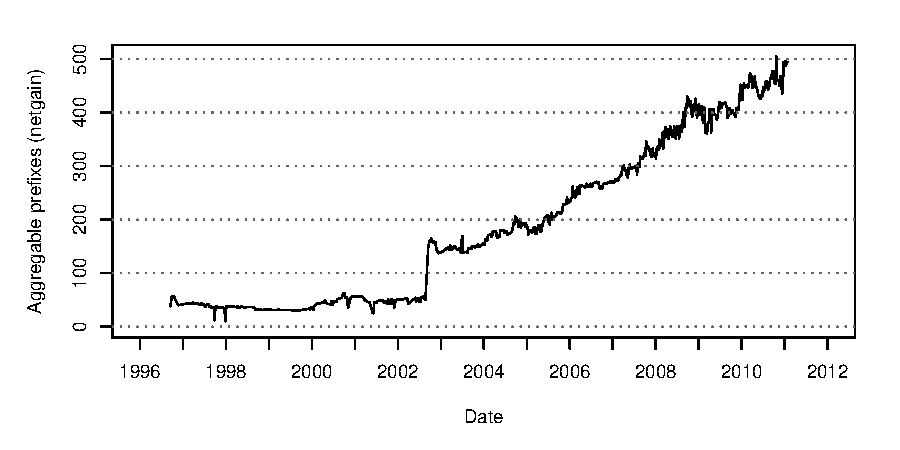
\includegraphics[width=6in]{figures/acr_netgain_time_min.pdf}
    \vspace{-2em}\\
    \caption{A plot of the minimum netgain required to appear on the CIDR Report over time.}
\end{centering}
\end{figure}

\begin{figure}[H]
\begin{centering}
    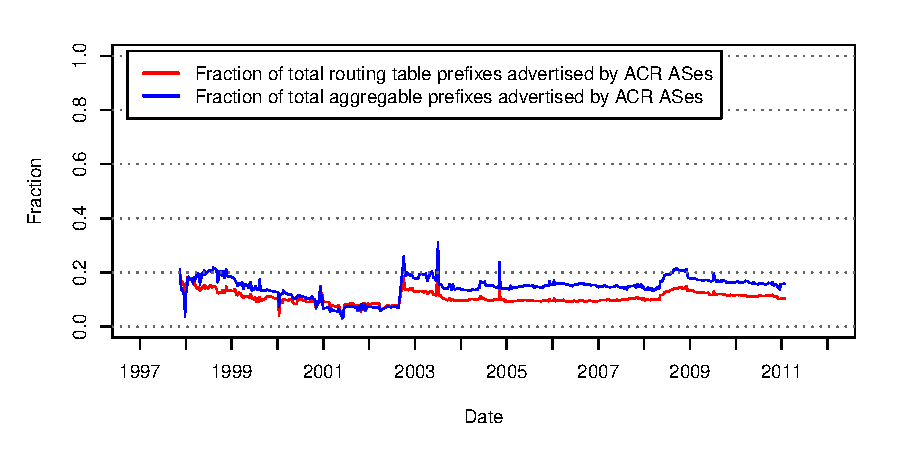
\includegraphics[width=6in]{figures/acr_gcr_netcompare.pdf}
    \vspace{-2em}\\
    \caption{Plots of the fractions of total prefixes and total aggregable prefixes in the routing table that are advertised by ASes appearing on the CIDR Report. \emph{Clarify methodological differences between ACR and GCR that should be noted in considering the validity of these plots.}}
\end{centering}
\end{figure}

\begin{figure}[H]
\begin{centering}
    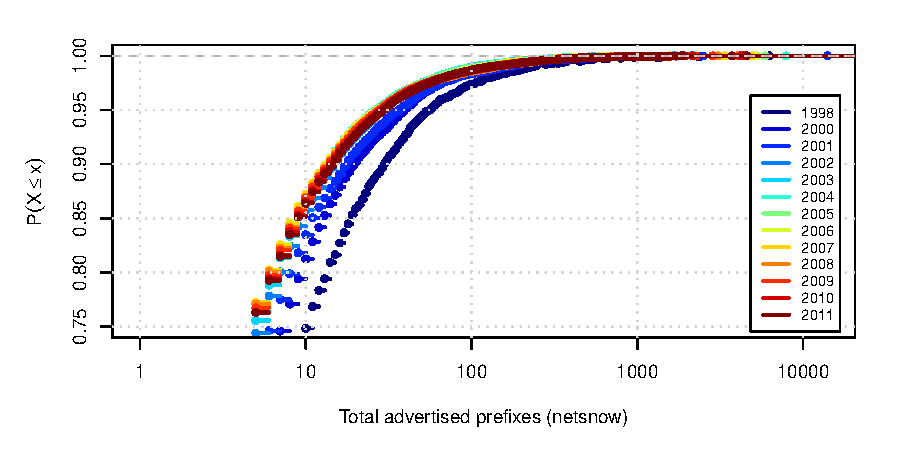
\includegraphics[width=6in]{figures/netgain_netsnow_cdf_gcr.pdf}
    \vspace{-2em}\\
    \caption{This one isn't particularly useful \fbox{and should probably be removed}, but it illustrates the movement after 2000 to more networks announcing fewer prefixes.}
\end{centering}
\end{figure}



\section{Analysis of AS behavior after appearing on the CIDR Report}

blah blah blah blah

\begin{figure}[H]
\begin{centering}
    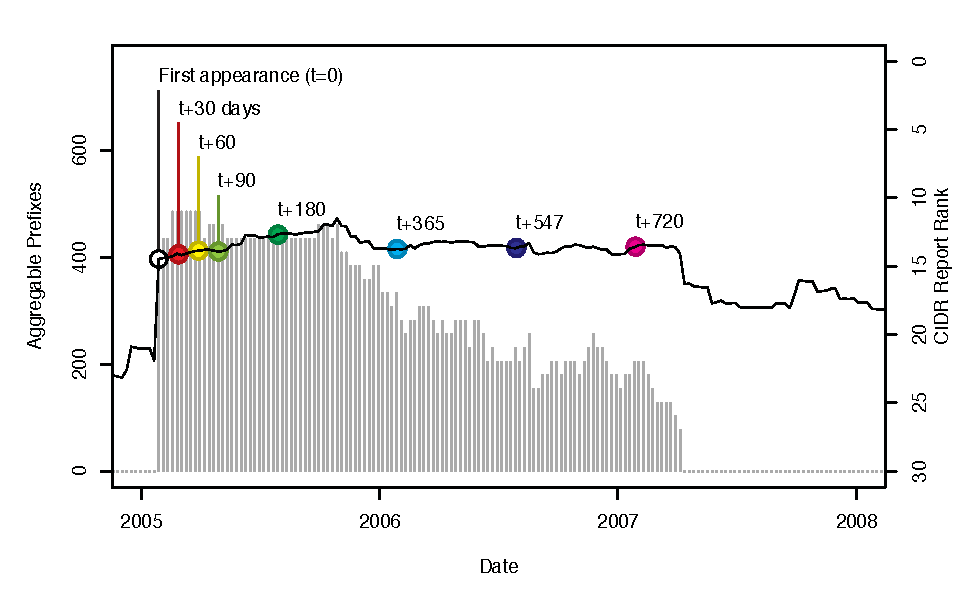
\includegraphics[width=6in]{figures/single_as.pdf}
    \vspace{-2em}\\
    \caption{Measurement methodology explanation (AS 3602).}
\end{centering}
\end{figure}


\subsection{Implementation Accuracy}

blah blah blah blah

\begin{figure}[H]
\begin{centering}
    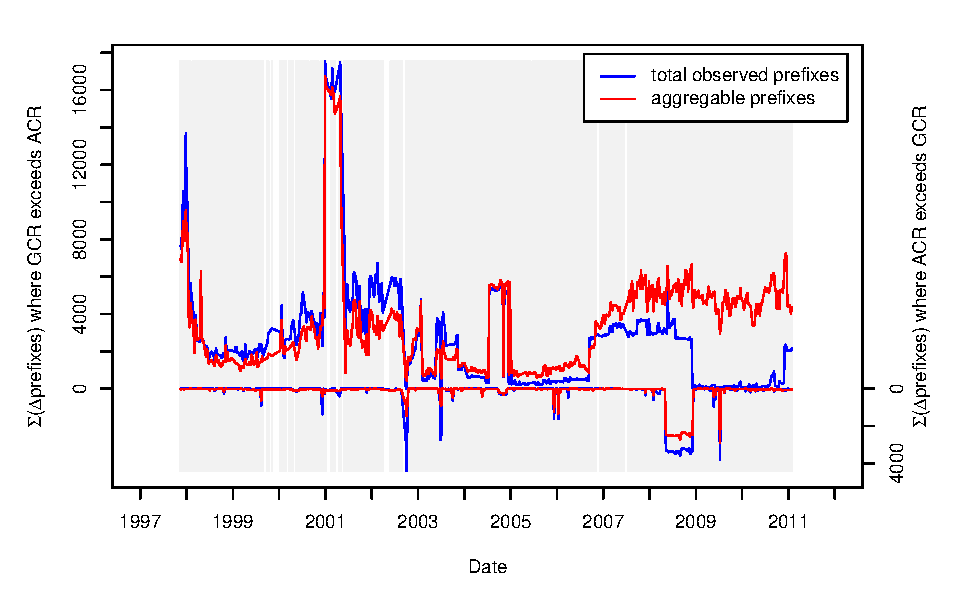
\includegraphics[width=6in]{figures/cidr_report_validity_prefix_error.pdf}
    \vspace{-2em}\\
    \caption{Differences in prefix counts between authoritative (ACR) and generated (GCR) CIDR Reports over time.}
\end{centering}
\end{figure}

\begin{figure}[H]
\begin{centering}
    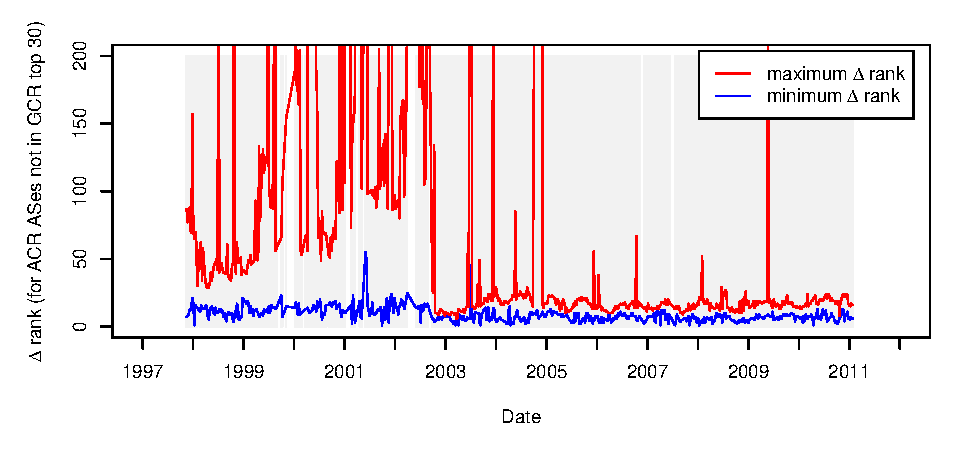
\includegraphics[width=6in]{figures/cidr_report_validity_rank_error.pdf}
    \vspace{-2em}\\
    \caption{Minimum and maximum differences in ASes ranked in the top 30 on the ACR but not in the top 30 on the GCR.}
\end{centering}
\end{figure}

\begin{figure}[H]
\begin{centering}
    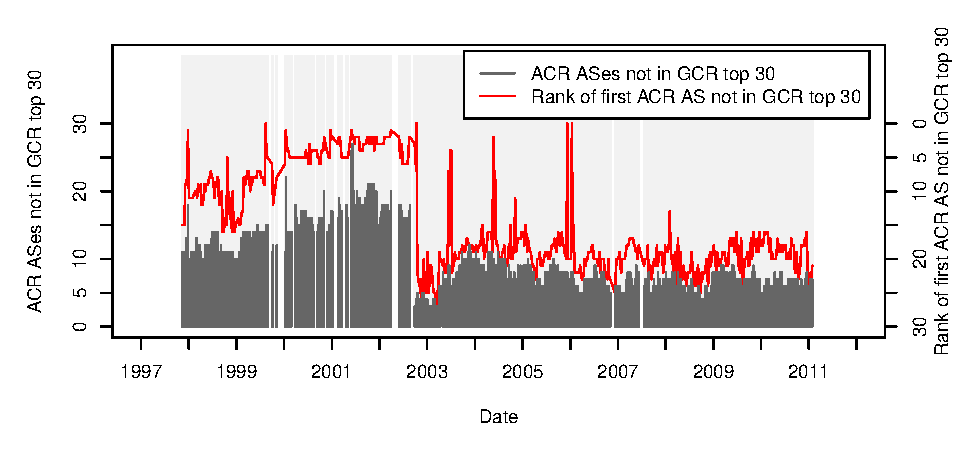
\includegraphics[width=6in]{figures/cidr_report_validity_top30_error.pdf}
    \vspace{-2em}\\
    \caption{The number and first rank of ASes in the treatment group (top 30) of the ACR that are not in the treatment group of the GCR over time.}
\end{centering}
\end{figure}

\fbox{plot deaggregation factor too -- 1 / (1 - aggfrac) or total/(total-aggregable)!!}

\subsection{Interpretation}

In spite of seeing aggregation behavior relative to the control, the total number of routes in the routing table does not drop over time, suggesting that old people are replaced by new ``bad guys'' or new entrants. Cittadini's study suggests that the proportion of ``bad guys'' remains the same over time (the people that would show up on the CIDR Report), suggesting the rolling-over bad guy theory.

OR. The table just grew less quickly than it otherwise could have, but we can't examine the counterfactual world...?

Rolling-over bad guy theory would be supported by the rate of growth of new ASes on teh CIDR Report?

Arthur suggests looking at the fraction (\# of /24s / \# of prefixes in the routing table) per AS or for the entire routing table, over time

What do Cittadini's observations mean for my analysis of the later repport where people are far more deaggregated

\subsection{Validity}
It was an oversight that I didn't measure behavior of ASes before their appearance on the CIDR Reprot. However, because appearance is determined based on netgain behavior means this is likely as not as huge a challenge to validity as I expected. I still need to be concerned that appearance didn't occur because someone else got less bad, but in such a case one's aggregation fraction would be at best flat, not decreasing to start (or they should've appeared earlier).

% valdiity notes
% - look at CDF of population elligible to be control
% CIDR Report overall behavior notes
% -> SELECT * FROM get_cumulative_ecr_asns();
% -> SELECT * FROM cumulative_gcr_as_counts;

%%%%%%%%%%%%%%%%%%%%%%%%%%%%%%%%%%%%%%%%%%%%%%%%%%%%%%%%%%%%%%%%%%%%%%%%%%%%%%%%

%ANALYSIS
%
%- Available data/data overview
%	- plot 'h' plots of available data
%	- plot total prefixes in the total table (Routeviews) and in the report (CIDR Report) to see that there aren't any discontinuities
%
%- Accuracy/error of my implementation of the CIDR Report
%
%- Visualization of aggregate behavior and general characteristics (in particular stratification at the top of the CIDR Report)
%    - Definition of metrics used in the analysis
%        - rank on CIDR Report (order by netgain)
%        - absolute/delta netgain
%        - relative/delta netgain (relative to netsnow)
%    - CDFs by AS appearnace
%    - CDFs by rank
%
%    - Summary/general statistics and characteristics of behavior over time (time series?), across and within groups, etc. (p62)
%
%- AS Behavior after appearing on the CIDR Report
%	- Distribution of AS behaviors from T=0, T=+1 month, 3 m, 6m, 1y, 2y, etc.
%		- all appearances on the CIDR Report
%		- no appearance/randomly selected control
%		- appearances that actually had behavior changes observed
%	- slice by date (NOT by rank on CIDR Report), and by netsnow
%
%- Variance in views of data from different peers
%- for different origin ASes that appear on the CIDR Report
%- across the entire routing table
%
%////////////////////////////////////////////////////////////////////////////////
%////////////////////////////////////////////////////////////////////////////////
%////////////////////////////////////////////////////////////////////////////////
%
%DISCUSSION
%
%Discussion of the design assumptions, and the sensitivity of the CIDR Report to those assumptions
